% !TeX spellcheck = cs_CZ
\begin{example}
  \textbf{Levitační elektromagnet}: Určeme indukované napětí na svorkách cívky levitačního 
  elektromagnetu podle obr \ref{teo:fig012}.
  
   {\centering
    \captionsetup{type=figure}
    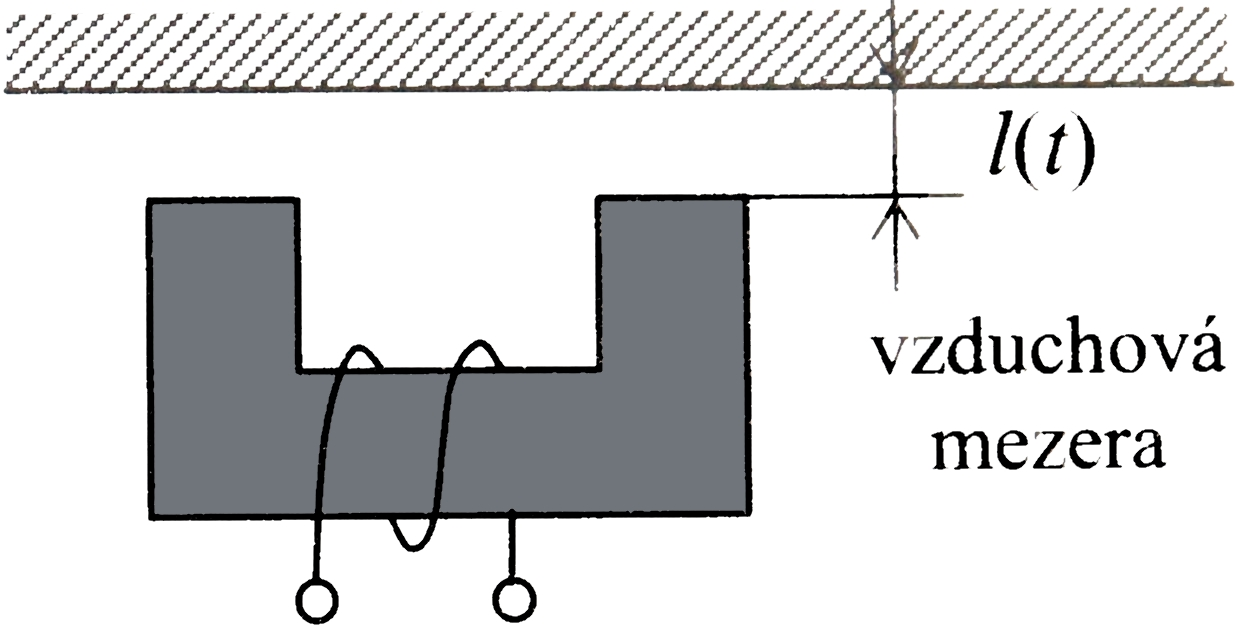
\includegraphics[width=0.6\linewidth]{teo_fig012.jpg}
    \captionof{figure}{Levitační elektromagnet jako příklad nelineárního parametrického 
               magnetického obvodu. (\cite[s.~161]{Patocka4})}
    \label{teo:fig012}
  \par}
  Z obrázku je zřejmé, že parametrem \(p(t)\) je délka \(l(t)\) vzduchové mezery. Tuto délku 
  dosadíme do rovnice (\ref{TEO:eq048}) namísto \( p(t)\):
  \begin{align}\label{TEO:eq076}
    u(t) &= \pder{\Psi[i, l]}{i}\der{i(t)}{t} + \pder{\Psi[i,l]}{l}\der{l(t)}{t}  \nonumber \\
         &= L_d[i,l]\der{i(t)}{t} + K_v[i,l]v(t)\,.
  \end{align}
  Indukované napětí levitačního elektromagnetu obsahuje dvě složky: první je úměrná derivaci proudu 
  a odpovídá napětí na diferenciální indukčnosti, druhá je úměrná vertikální rychlostí jha (tato 
  složka vzniká při pohybu i v případě, že proud cívkou udržujeme na \emph{konstantní} hodnotě!

\end{example}


